\chapter{Implementation}\label{C:imp} 

% \begin{wrapfigure}{r}{0.3\textwidth}
%  \begin{center}
%   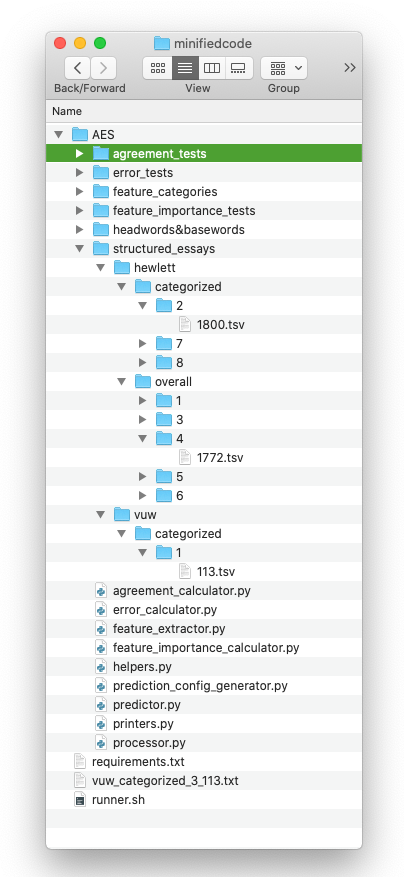
\includegraphics[width=0.25\textwidth]{pngs/struct.png}
%  \end{center}
%  \caption{Project Structure}
% \end{wrapfigure} 


\section{Development}

Initial programs were made using google-colab. This platform was beneficial in the exploration stage for programmatically investigating Natural Language Processing and Machine Learning. Following this, all implementation was done with Python in Visual Studio Code. Several libraries have been incorporated, such as Natural Language Toolkit, Language Check, Text Stat, Pandas, Matlab, Sklearn. Executions were orchestrated using Bash. Amazon's Elastic Cloud Compute (EC2) service was also used for executions. Amazon Elastic Compute Cloud is a part of Amazon.com's cloud-computing platform, Amazon Web Services, which allows users to rent virtual computers to run their computer applications.

\subsection{Structure}

The project's root is the "AES" folder, the requirements.txt, and the "runner.sh" which is the batch job orchestrator bash script. Also, all execution log files will appear at this level of the project. My reason for only having these files at this level is that the project is more runnable than a codebase. So all the things you need to execute any component can be done from here, and all log files will appear here without the clutter or mechanics of the python files that do the automatic scoring getting in the way.

Inside the AES folder is where all of the python code files, data, and artifacts live. The folders at this level are split into categories based on the artifacts that the project produces or consumes, such as; agreement tests, feature categories, headwords, and baseboards. Also, at this level are all of the python files. Again, this is pure to accommodate working with multiple files in Python. Splitting up the code as much as possible was a priority of mine as I wanted to keep the code abseils as manual as possible so that each opponent was easy to understand and there develop and debug. Although this does mean that there are several main files all at one place in eh director, this was worth it as I wanted to avoid creating a monolith. Again this was for my benefit as well as the future students of this project. Additionally, having well-defined separated responsibilities allows for a more straightforward explanation of the system to non-technical stakeholders. The location or folder structure of most artifacts, can be seen in the figure. I made this early design choice to standardise the general structure for any given dataset, of any version, being run against any component. This was a benefit as there is a lot of cross-pollination of the component ts. As they all produce and consume different artifices for each other. So having some unified rules around this was helpful. This is primarily due to the nature of my modularised system, where each component is frequently importing and exporting things.

% \begin{wrapfigure}{r}{0.5\textwidth}
%  \begin{center}
%   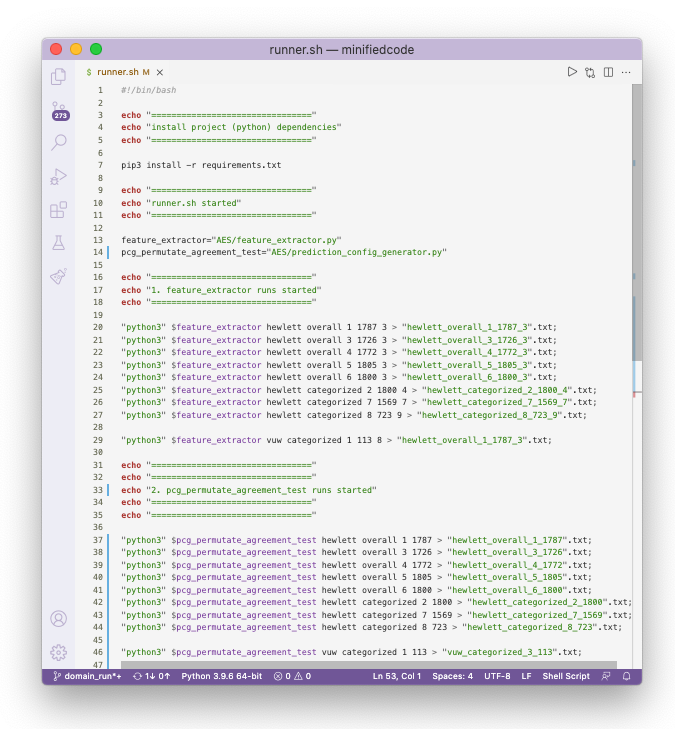
\includegraphics[width=0.55\textwidth]{pngs/runner.png}
%  \end{center}
%  \caption{Batch Job: Multiple Executions}
% \end{wrapfigure}

\subsection{Executions}
An execution can be thought of as running a component against a dataset. For example, common execution goals include running The Feature Extractor against the VUW EPP data to produce Feature Categories or running The PCG, The Predictor, and The Agreement Calculator against the Hewlett data to produce Agreement Measures. Often multiple executions are grouped and commenced with a single command, just like how a batch job might be done. A batch job can be considered a predefined group of processing actions with little or no interaction between the user and the system. In our case, this was often to run multiple datasets through the feature extractor, predictor, and agreement calculator. 

\subsection{Workflow}
The workflow for conducting an execution is described in the following diagram.

% \begin{figure}[h]
%   \centering
%   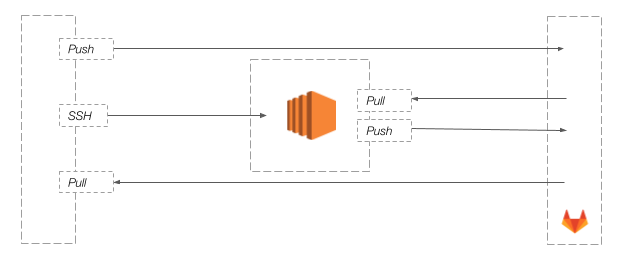
\includegraphics[width=.6\linewidth]{pngs/workflow-updated.png}
%   \caption{Workflow}
%   \label{Fig:Data1}
% \end{figure}

\paragraph{Push}
This step is required to provide the EC2 instance with the relevant resources that it may require for a proposed execution. These resources are committed and pushed from the local machine and then are retrieved or pulled from git before an execution. For example, if the proposed execution is to generate features for a new dataset, this would require committing and pushing the respective dataset's TSV file, provided it is in the correct location.

\paragraph{SSH} Once connected to the cloud instance. You can first pull from the remote to receive the newest version of the project on the instance. Following this, you can execute the runner script, which will execute predefined executions. After the bash script has been completed, you can then commit the newly created artifacts and push them to the remote to update them with the newly produced artifacts. While the bash script or runner is executing, you can observe the status of each job by viewing the associated log file. 

This was made possible by incorporating extensive logging for all types of execution. The motivation and gains of this are discussed in the following sections.

As many components interact, it was beneficial to have some form of sanity checking to help mitigate elementary mistakes or impossibilities that might be unclear when programming or are based on invalid assumptions. In addition, having this level of visibility helped to ensure the system was operating as I expected. This was especially helpful when ensuring intended permutations were being made, which datasets were being used, as developing and validating this process could get quite overwhelming otherwise.

Having these extensive logs also provided more information when troubleshooting or investigating bugs by providing more information. As well as this, for most systems of its maturity, the time to implement some form of incremental run-state backup system is not worth it. In most cases, for systems of this maturity, if the system is running a job and it encounters an error, the system will crash entirely, and its current task's progress will be lost. And unfortunately, until that problem is resolved, the same task will continue to fail until it is directly attended to.

Additionally, I chose to export this log data to a file as, over time, the amount of information I was outputting exceeded the console's memory limit. As well as this, it was tough to retrieve log statements when running in the cloud after exiting an ssh session for a process executed. However, it also meant that I could quickly and conveniently review a job's status post-run.

\paragraph{Pull} Once all executions have been completed or when you reconnect to the server, you can commit and push all new artifacts to the remote. Then you can exit the SSH session, and from your local machine, pull from the remote to receive all the newly produced artifacts.

\section{The Feature Extractor}

The Feature extractor can be broken down into the following main stages.

\paragraph{1. Initialise } In the Initialisation stage, one of the first things the AES will do is load any pre-existing resources that it may require, such as the headwords list, stop words list, and POS trigrams. Also, in this step, the system will initialize any necessary data structures, such as the lists for each feature category.

\paragraph{2. Import} In the import stage, the system will read and translate the relevant essay TSV into a two-dimensional array. The location of the relevant structured essay, as mentioned previously, will be derived from the run parameters.

\paragraph{3.} Then, for every essay, it will:

\paragraph{3.1. Process Identifiers} Here, the feature extractor will process the essays identifiers to all feature categories.

% \begin{wrapfigure}{l}{0.6\textwidth}
%  \begin{center}
%   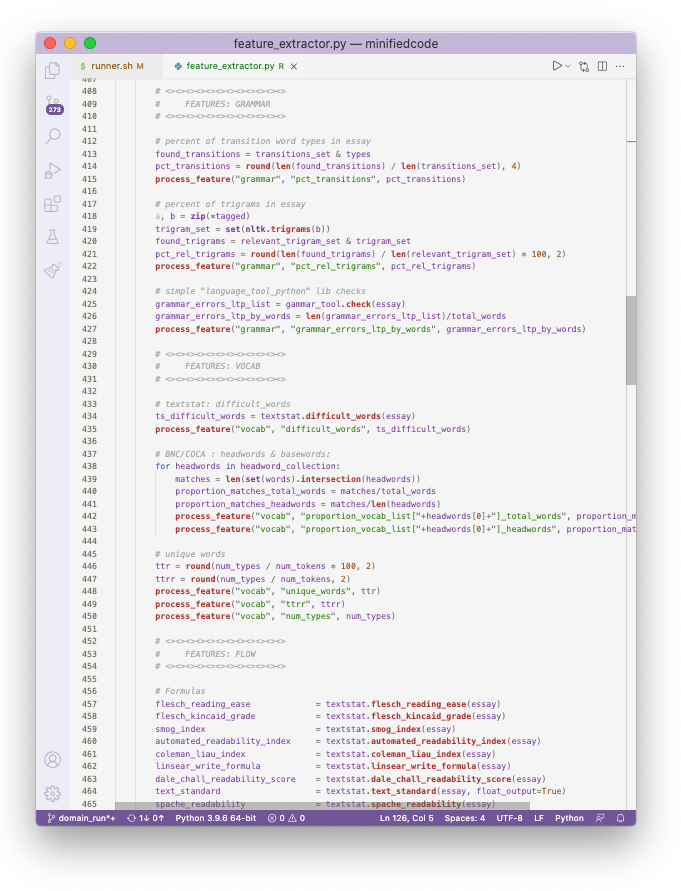
\includegraphics[width=0.55\textwidth]{pngs/feature-extract-code.png}
%  \end{center}
%  \caption{The Feature Extractor}
% \end{wrapfigure}

\paragraph{3.2. Process The Features} Processing a feature is done by performing a predefined calculation and then inputting the result of that calculation into the "processing" method along with a category. This method will then add the value or result of the feature to a list for the specific category and the overall category. This was done simply as a naive approach to categorising. Going forward, this should be updated. 

\paragraph{4. Export Feature Categories} Lastly, the Feature Extractor will translate the categorised data structures into separate TSV fikes. In order to produce feature categories containing all essays with only the feature values specific to themselves.

\subsection{Feature Importance Tests}

The future tests work by comparing the overall future category, which contains all features, to every categorical score using many helper methods from sklearn similar to the prediction component. 

% \begin{wrapfigure}{r}{0.5\textwidth}
%  \begin{center}
%   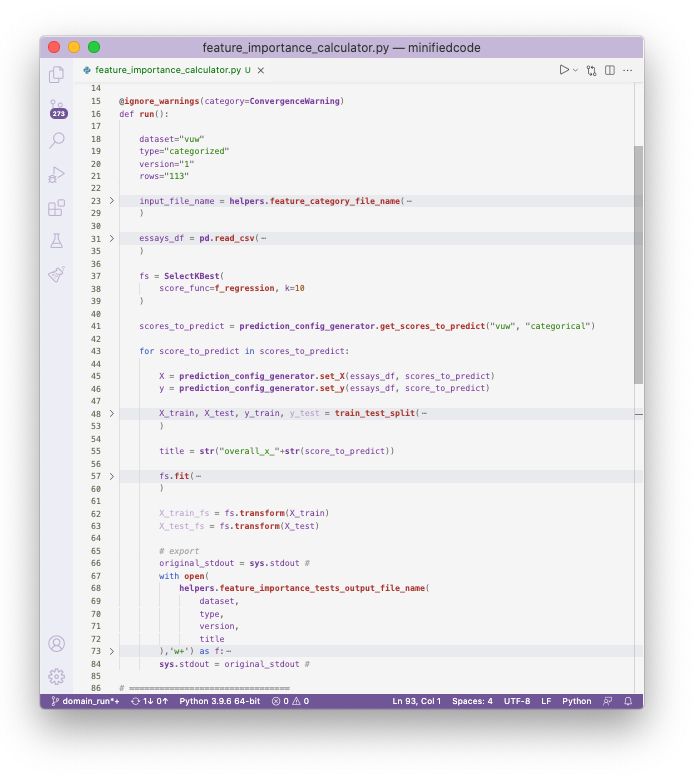
\includegraphics[width=0.48\textwidth]{pngs/feature-importance-code.png}
%  \end{center}
%  \caption{Feature Importance Tests}
% \end{wrapfigure}

\section{The Predictor}

From a programmatic perspective, the prediction component is relatively simple as it can be done in one line of code using the sklearn library. Therefore, in the final solution, this component will use the most optimal pre-trained model, for a category, from an imported ".pkl" file. However, for the duration of this project, these models only needed to persist at run time for a single execution. Therefore they did not need to be exported. 

% \begin{wrapfigure}{r}{0.5\textwidth}
%  \begin{center}
%   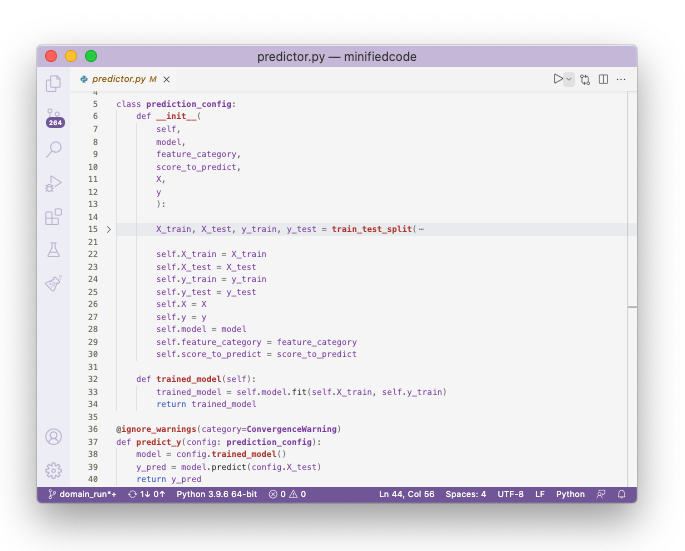
\includegraphics[width=0.48\textwidth]{pngs/predictor-code.png}
%  \end{center}
%  \caption{The Predictor}
% \end{wrapfigure}

\subsection{The Prediction Configuration Generator}

The Prediction Configuration Generator has two main methods. Permeate, and Run. They use the Prediction Configuration class, which stores a model, feature category, score to predict, and other fields. 
Having this simple class is super helpful for retaining an intended test's information.

The Permutate method mainly consists of a triple nested loop that loops through predefined models, feature categories, and scores to predict. The list of models remains the same for all execution types or configurations—however, the feature categories and scores to predict can vary depending on the execution params. For example, the scores to predict list for an "overall" run type only consist of the overall score. Each inner iteration will train a model, produce predictions, and compare them to the human-produce scores to produce agreement measures. One thing to note in this method is the outlier function. 

% \begin{figure}[h]
%   \begin{minipage}{0.48\textwidth}
%   \centering
%   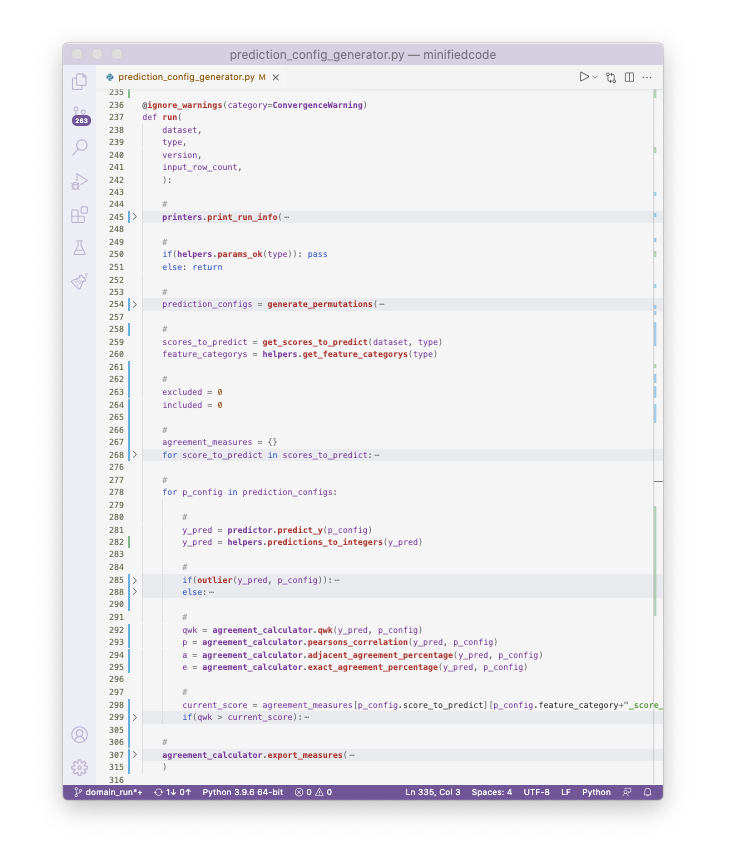
\includegraphics[width=.7\linewidth]{pngs/pcg.png}
%   \caption{Interpolation for Data 1}\label{Fig:Data1}
%   \end{minipage}\hfill
%   \begin{minipage}{0.48\textwidth}
%   \centering
%   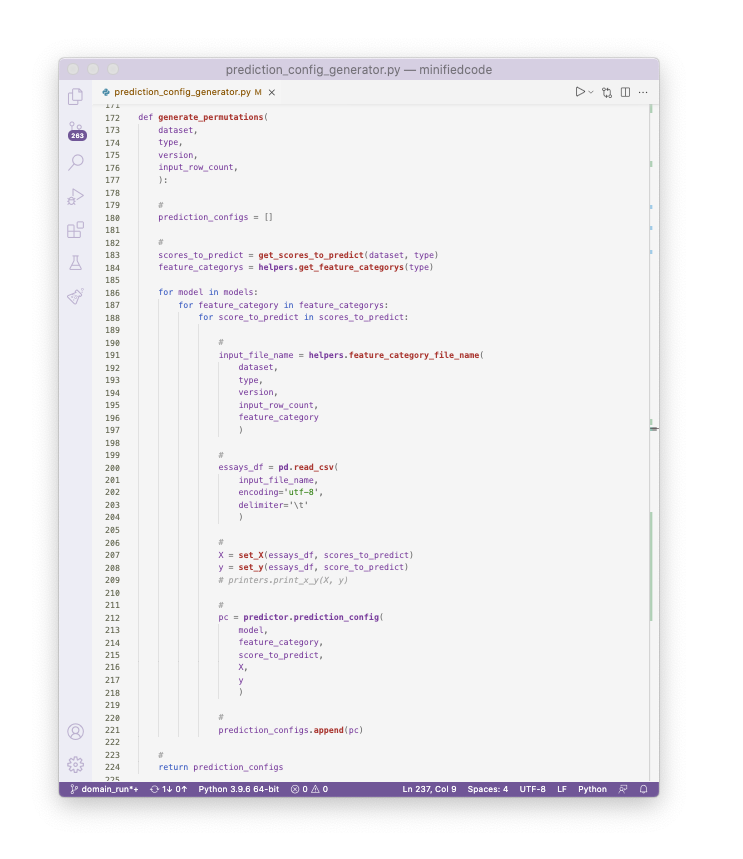
\includegraphics[width=.7\linewidth]{pngs/permutations.png}
%   \caption{Interpolation for Data 2}\label{Fig:Data2}
%   \end{minipage}
% \end{figure}

The motivation behind this was to avoid processing any tremendous prediction values generated by the computer. Not only did this take a very long time, but it also meant that Prediction Configuration was very, wildly inaccurate anyway. So it did not need to be consumed by the agreement calculator and component to the current best QWK because it would not be a suitable candidate for having the best QWK. 

The way these unusually high values are moderated is simply by calculating the mean of the prediction values list and comparing this to the mean of the actual human-generated scores list. If the mean is too big, the triple nested loop will end that iteration and start the logical next iteration.

To validate this, to make sure that I was not removing valuable test results. I implemented an "excluded "count and divided this by the size of the precision values list to get the percentage of Prediction Configurations being ignored. I have just left this debugging code in the system, and for all run's observed, the ignored configurations are a relatively small proportion.

\subsection{The Agreement Calculator}

The Agreement Calculator calculates the following measures: Quadratic Weighted Kappa, Pearson correlation coefficient, Adjacent Agreement Percentage, Exact Agreement Percentage. The logic and maths of the first two are mainly outsourced to sklean. The following two are both created manually. Most of these metrics do some mathematical operations on the human given scores and the computer-generated scores. 

% \begin{wrapfigure}{r}{0.5\textwidth}
%  \begin{center}
%   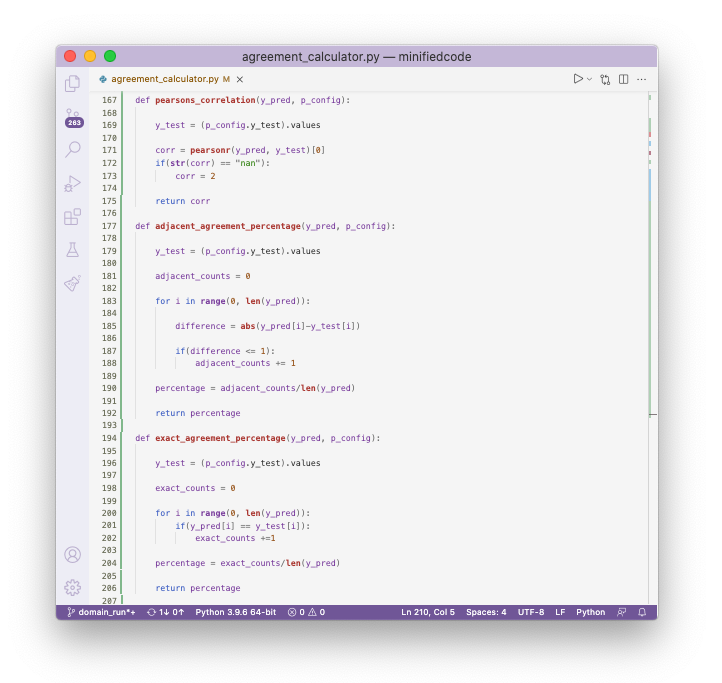
\includegraphics[width=0.48\textwidth]{pngs/agreement-calc.png}
%  \end{center}
%  \caption{The Agreement Measures}
% \end{wrapfigure}

In the case of the adjacent-agreement measure, this is calculated by comparing these two values, calculating the absolute difference between them, checking if the difference is one (or less), and if so, incrementing the adjacent count variable by 1. This is done until all pairs of values are checked. Then, following this, a percentage is calculated by dividing the adjacent counts by the total pairs. In the case of the exact agreements, the producer is very similar. However, we check whether both values are the same instead of calculating a difference between the computer and human-generated scores. If they are, a counter is incremented, and a percentage out of all predictions is calculated from this, like the other measure.
